\iffalse
\documentclass[10pt, a4paper]{article}
\usepackage[a4paper,outer=1.5cm,inner=1.5cm,top=1.75cm,bottom=1.5cm]{geometry}

%\twocolumn
\usepackage{graphicx}
\usepackage{karnaugh-map}
\usepackage{tabularx}
\usepackage{hyperref}
\usepackage[utf8]{inputenc}
\usepackage{amsmath}
\usepackage{physics}
\usepackage{amssymb}
\newcommand{\myvec}[1]{\ensuremath{\begin{pmatrix}#1\end{pmatrix}}}
\let\vec\mathbf

\begin{document}
\title{Optimization Assignment}
\author{Name:A.Gowri Priya\and Email :  \url{gowripriyaappayyagari@gmail.com}}
%\{ Wireless Communication (FWC)}
\date{}
\maketitle
  \section{Problem}
  \fi
A factory makes tennis rackets and cricket bats. A tennis racket takes 1.5 hours of machine time and 3 hours of
craftman’s time in its making while a cricket bat takes 3 hour of machine time and 1 hour of craftman’s time. In a
day, the factory has the availability of not more than 42 hours of machine time and 24 hours of craftsman’s time.
\begin{enumerate}
	\item What number of rackets and bats must be made if the factory is to work at full capacity?
	\item  If the profit on a racket and on a bat is Rs 20 and Rs 10 respectively, find the maximum profit of the factory when
it works at full capacity.
\end{enumerate}
\solution
The given information is summarized in Table
		\ref{table:12/12/2/3}.
\iffalse
\section{Solution}
Let's assume that

\begin{center}
Number of Tennis rackets be x\\
Number of Cricket Bats be y\\
\end{center}
\fi
\begin{table}[!ht]
	\centering
\begin{tabular}{|c|c|c|c|c|}
	\hline
	\textbf{Item}&\textbf{Number}&\textbf{Machine hours}&\textbf{Craftman's hours}&\textbf{Profit}\\
	\hline
	Tennis Rackets&x&1.5&3&$Rs.20$\\
	\hline
	Cricket Bats&y&3&1&$Rs.10$\\
	\hline
	Maximum time available& &42&24\\
	\hline
\end{tabular}
	\caption{}
		\label{table:12/12/2/3}
\end{table}
	\begin{figure}[!ht]
		\centering
		\includegraphics[width=\columnwidth]{12/12/2/3/figs/optm.png}
		\caption{}
		\label{fig:12/12/2/3}
  	\end{figure}
	\iffalse
According to question:

\begin{align}
 1.5x+3y \le 42 \\
=>3x+6y \le 84 \\
=>x+2y \le28
\end{align}
\begin{align}
\myvec{1&2}\myvec{x\\y}\le 28
\end{align}\\
Also,\\
\begin{align}
 3x+y \le 24 \\
\end{align}
\begin{align}
\myvec{3&1}\myvec{x\\y}\le 24
\end{align}\\
As we need to maximize profit,\\
Hence,function used here will be maximize Z\\
\begin{center}
profit on Tennis Racket=$Rs.20$\\
profit on Cricket Bat=$Rs.10$\\
Maximize Z=20x+10y\\
\fi
From the given information, the optimization problem can be expressed as
\begin{align}
	Z=\max_{\vec{x}}\myvec{20&10}\vec{x}
	\\
s.t. \quad \myvec{1&2\\3&1}\vec{x}\preceq \myvec{28\\24}
\\
\vec{x} \succeq \vec{0}
\end{align}
\iffalse
\begin{align}
  x \ge 0, y \ge 0
\end{align}
\begin{align}
\myvec{1&2}\myvec{x\\y}\le 28
\end{align}\\
\begin{center}
\begin{tabular}{|c|c|c|}
	\hline
	x&0&14\\
	\hline
	y&14&7\\
	\hline
\end{tabular}\\
\end{center}
\begin{align}
\myvec{3&1}\myvec{x\\y}\le 24
\end{align}\\
\begin{center}
\begin{tabular}{|c|c|c|}
	\hline
	x&2&8\\
	\hline
	y&18&0\\
	\hline
\end{tabular}\\
\end{center} 
\begin{center}
	\fi
	From Fig. 
		\ref{fig:12/12/2/3}, the values at the corner points are
		obtained in 
Table
		\ref{table:12/12/2/3/1}.

	\begin{table}[!ht]
		\centering
\begin{tabular}{|c|c|}
	\hline
	\textbf{Corner points}&\textbf{Value of Z}\\
	\hline
	(0,14)&140\\
    \hline
	(4,12)&200\\
	\hline
	(8,0)&160\\
	\hline
\end{tabular}
		\caption{}
		\label{table:12/12/2/3/1}
\end{table}
At full capacity,
\begin{align}
	\vec{x}&=\myvec{4\\12},
	\\
	\implies Z&=\myvec{20&10}\myvec{4\\12}
	\\
	&=200
\end{align}
This is verified using cvxpy.
\iffalse
$\therefore$Maximum profit=Rs.\\
\section{Construction}
\begin{figure}[h]
\includegraphics[scale=0.5]{optm.png} 
\end{figure}
\section{Execution}
Verify the above proofs in the following code.\\
\framebox{
\url{https://github.com/gowripriya-2002/FWC/blob/main/Optimization/Basic/code/opp.py}}	
\bibliographystyle{ieeetr}
\end{document}
\fi
